\graphicspath{{./images/}}
% Configure style


\titleformat{\section}
{\normalfont\fontfamily{phv}\fontsize{10}{0}\bfseries}{\thesection}{1em}{}
\section{Transformer Models}
\renewcommand\labelitemi{{\boldmath$\cdot$}}
\setlist{nolistsep}
\begin{itemize}[noitemsep]
      \item Natural Language Processing (NLP)
            \begin{itemize}[noitemsep]
                  \item Tasks
                        \begin{itemize}[noitemsep]
                              \item \textbf{Classifying whole sentences}: Getting the sentiment of a review, detecting if an email is spam, determining if a sentence is grammatically correct or whether two sentences are logically related or not
                              \item \textbf{Classifying each word in a sentence}: Identifying the grammatical components of a sentence (noun, verb, adjective), or the named entities (person, location, organization)
                              \item \textbf{Generating text content}: Completing a prompt with auto-generated text, filling in the blanks in a text with masked words
                              \item \textbf{Extracting an answer from a text}: Given a question and a context, extracting the answer to the question based on the information provided in the context
                              \item \textbf{Generating a new sentence from an input text}: Translating a text into another language, summarizing a text
                        \end{itemize}
                  \item Rise of LLMs
                        \begin{itemize}[noitemsep]
                              \item Perform a wide variety of the above language tasks without task-specific training
                              \item Scale, general capabilities, in-context learning, emergent abilities
                              \item Limitations:
                                    \begin{itemize}[noitemsep]
                                          \item Hallucinations
                                          \item Lack of true understanding
                                          \item Reflecting training data bias in outputs
                                          \item High computational and environmental costs
                                    \end{itemize}
                        \end{itemize}
            \end{itemize}
      \item Transformers are everywhere!
            \begin{itemize}[noitemsep]
                  \item NLP, Computer Vision, Audio Processing, Multimodal Models
                  \begin{lstlisting}
                    from transformers import pipeline

                    classifier = pipeline("sentiment-analysis")
                    classifier(
                        ["I've been waiting for a HuggingFace course my whole life.", "I hate this so much!"]
                    )

                    [{'label': 'POSITIVE', 'score': 0.9598047137260437},
                    {'label': 'NEGATIVE', 'score': 0.9994558095932007}]        
                  \end{lstlisting}
                  \item text-generation, text-classification, summarization, translation,
                        zero-shot-classification, feature-extraction, image-to-text, image-classification,
                        object-detection, automatic-speech-recognition, audio-classification,
                        text-to-speech, image-text-to-text
                  \item Model Hub: \url{https://huggingface.co/models}
            \end{itemize}
      \item How do Transformers work?
            \begin{itemize}[noitemsep]
                  \item 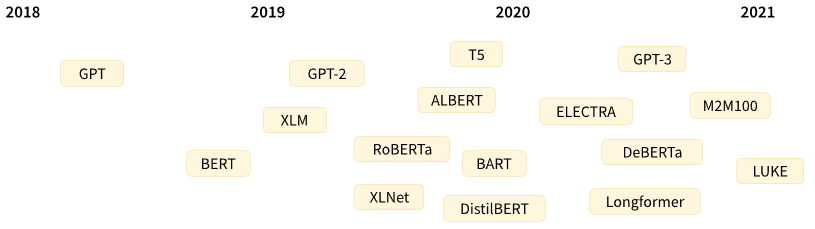
\includegraphics[height=0.27\linewidth]{transformers_chrono.png}
                  \item Carbon Footprint
                        \begin{itemize}[noitemsep]
                              \item CO2 = f(type of energy, training time, hardware, region)
                              \item Use pretrained models, fine-tuning, smaller experiments + debugging,
                                    literature review of hyperaparameter ranges, random search vs. grid search
                        \end{itemize}
                  \item Transfer Learning is the act of initializing a model with
                        pretrained weights, then fine-tuning it on a downstream task.
                        \begin{itemize}[noitemsep]
                              \item Pretraining objective: Predict the next word in a sentence
                              \item Pretraining objective: Guess the value of randomly masked words
                              \item Fine-tuning: Further training the model on a smaller,
                                    task-specific dataset
                              \item Always try to leverage a pretrained model first!
                        \end{itemize}
            \end{itemize}
      \item How Transformers solve tasks
            \begin{itemize}[noitemsep]
                  \item Language models are trained to predict the probability of a word given context of surrounding words
                        \begin{enumerate}
                              \item Masked language modeling (MLM): Randomly mask some tokens and train model
                                    to predict the original tokens based on surrounding context.
                                    This allows model to learn bidirectional context (i.e. BERT).
                              \item Causal language modeling (CLM): Train model to predict the next token in a sequence
                                    given all previous tokens (i.e. GPT).
                        \end{enumerate}
                  \item 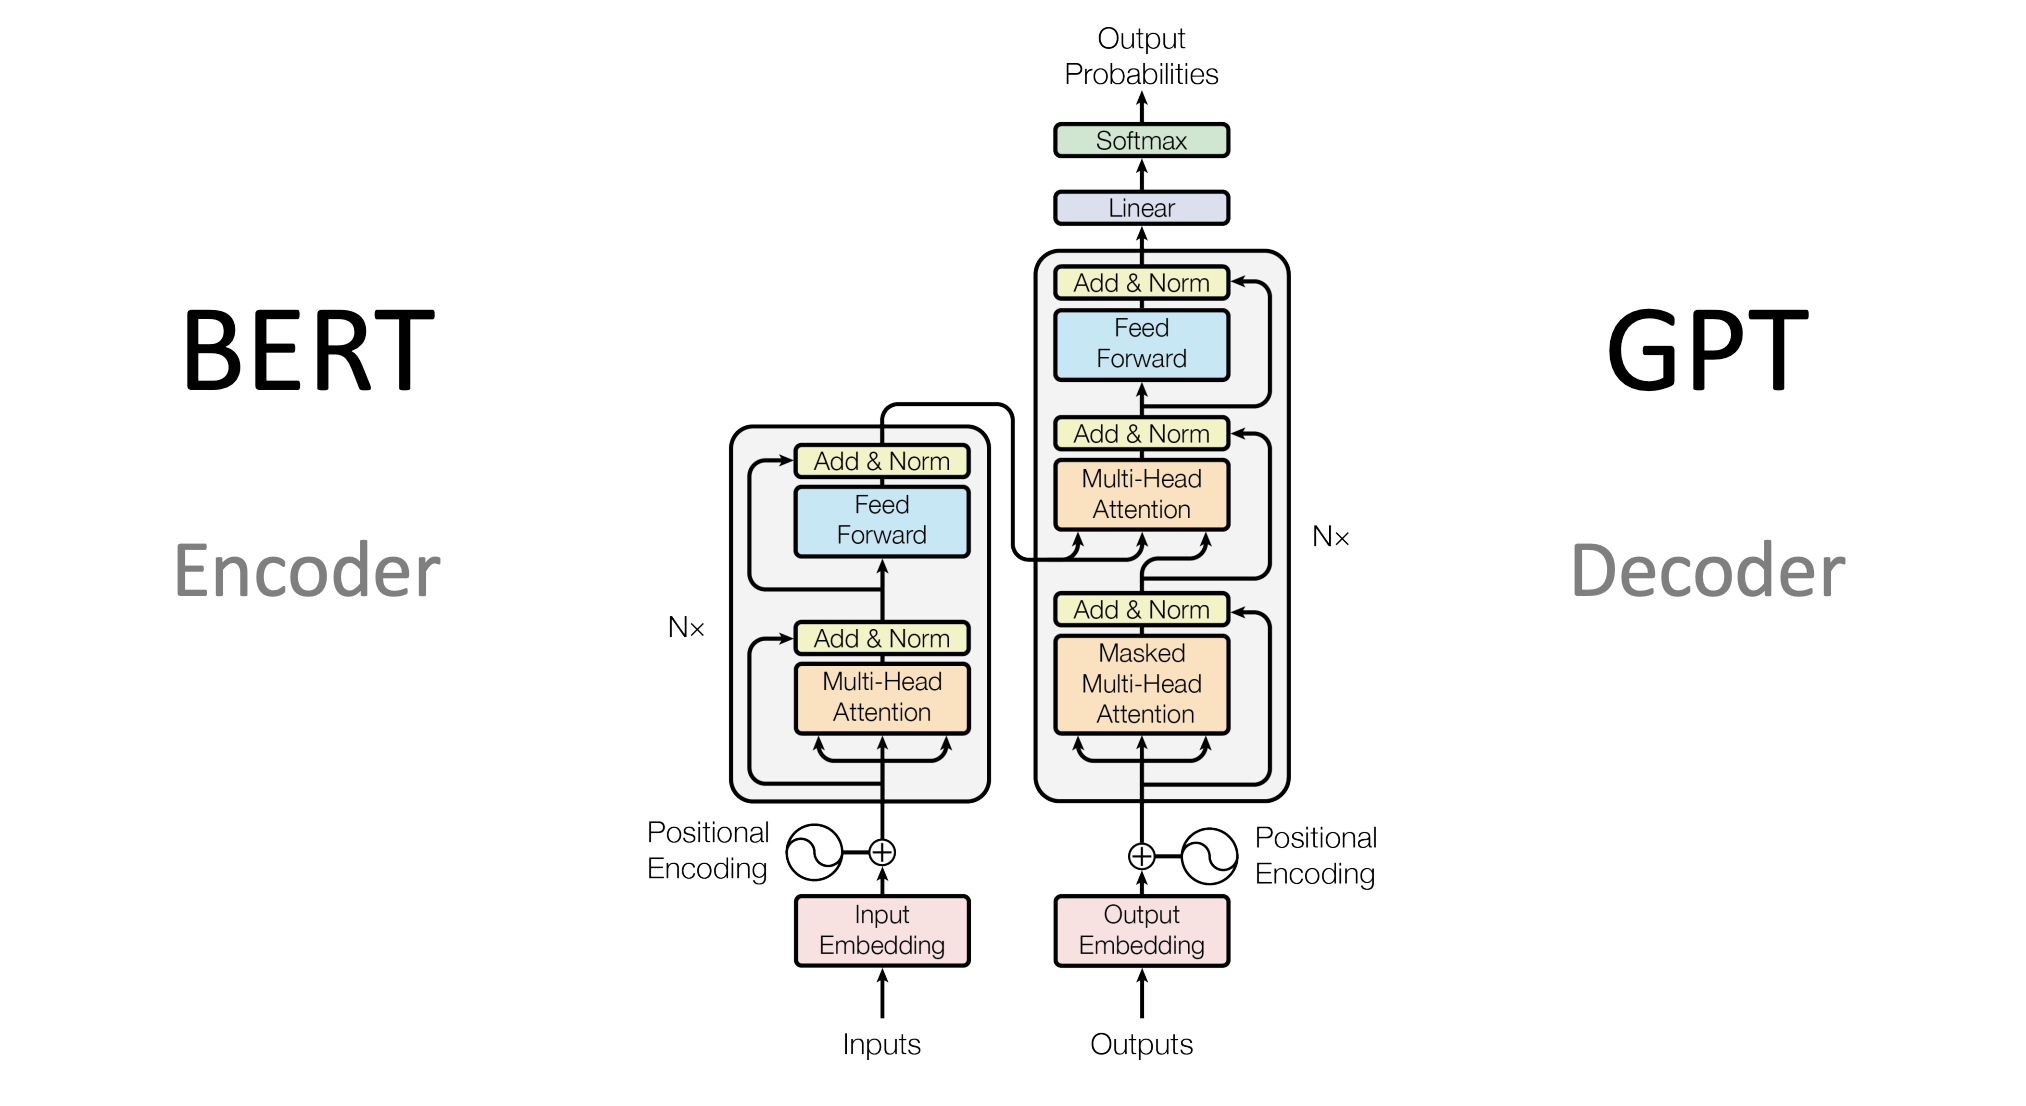
\includegraphics[height=0.5\linewidth]{transformers_architecture.png}
                  \item Types of language models
                        \begin{enumerate}
                              \item Encoder-only models (i.e. BERT): Understand context from both directions. For tasks
                                    requiring deep understanding of text, such as classification, NER, and Q\&A.
                              \item Decoder-only models (i.e. GPT): Process text from left-to-right.
                                    Great at text generation tasks such as sentence completion, creative writing,
                                    code generation.
                              \item Encoder-Decoder models (i.e. T5, BART): Combine both approaches. Great at
                                    sequence-to-sequence tasks like translation, summarization, and Q\&A.
                        \end{enumerate}
                  \item Tasks
                        \begin{itemize}[noitemsep]
                              \item Text Generation: output from decoder passed to language modeling head, which 
                              does linear transformation to convert hidden states into logits. Cross-entropy loss
                              calculated between shifted logits and labels to output most likely token
                              \item Text Classification: Pretrained BERT + sequence classification head 
                              (transforms hidden states into logits). Cross-entropy  between logits and labels to find
                              most likely label
                              \item  Token Classification: Pretrained BERT + token classification head (transforms
                              hidden states into logits). Cross-entropy loss between logits and each token to find 
                              most likely label 
                              \item Question Answering: Pretrained BERT + Span classifcation head (transforms hidden 
                              states into start and end logits). Cross entropy loss between logits and label position 
                              to find most likely span of text. 
                              \item Summarization: Pretrained BART + seq2seq language modeling head (linear transformation
                              to convert decoder hidden states into logits). Cross-entropy loss between shifted logits
                              and labels to output most likely token
                              \item BART encodes source language into an embedding, then decoder generates target language 
                              \item Speech and audio: Whisper model transcribes audio into text and does translation 
                              using encoder-decoder architecture. Whisper is trained on 680,000 hours of labled audio data 
                              \item Computer Vision: Two approaches
                                    \begin{itemize}[noitemsep]
                                          \item Vision Transformer (ViT): Splits image into patches, flattens them, and
                                                processes them as a sequence using transformer architecture
                                          \item Hybrid models (i.e. ConvNeXT): Use CNN layers to extract features 
                                                from images, then feed these features into transformer layers for 
                                                further processing
                                    \end{itemize}
                        \end{itemize}
            \end{itemize}
      \item Transformer Architectures 
            \item 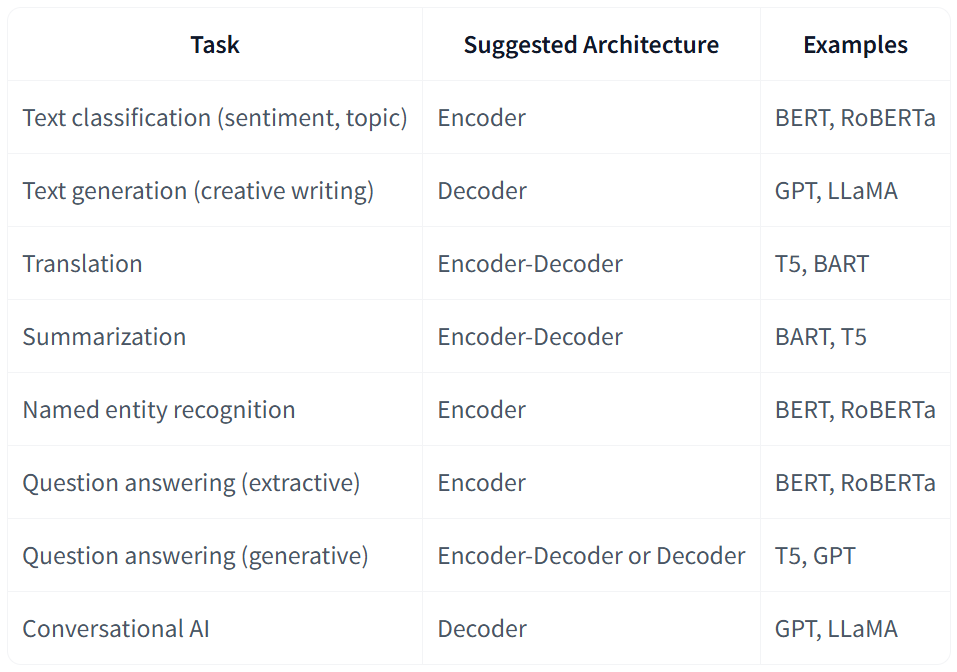
\includegraphics[height=0.5\linewidth]{transformer_architectures_table.png}
\end{itemize}